% !TEX root = ../thesis.tex

\chapter{Training und Test der Machine-Learning-Klassifikatoren}

\paragraph{Ausblick:}
Dieses Kapitel gibt einen detaillierten Einblick in das Training der Machine-Learning-Klassifikatoren. Dazu werden zunächst die verwendeten Klassifikatoren und deren initiale Auswahl erläutert. Anschließend werden der Trainingsprozess sowie die zum Einsatz kommenden Softwarewerkzeuge beschrieben.
\\
\hrule

\section{Auswahl der Werkzeuge und Klassifikationsalgorithmen}

Durch die Wahl der Programmiersprache Python, war die Entscheidung zur Auswahl eines Machine-Learning-Werkzeugs bereits absehbar. Zur Anwendung kommt die Python-Library scikit-learn\footnote{\href{https://scikit-learn.org/}{https://scikit-learn.org/}}, die im Jahr 2007 von Pedregosa et. al entwickelt wurde \cite{scikit}. Das Werkzeug bietet eine große Auswahl an Machine-Learning-Algorithmen für überwachtes und unüberwachtes Lernen und ermöglicht darüber hinaus eine einfache Implementation sowie eine einfache Einbindung weiterer Python-Libraries, wie beispielsweise die Matplotlib zur Erstellung von mathematischen Darstellungen \cite{scikit}.

Ebenfalls wird der WEKA-Workbench\footnote{\href{https://www.cs.waikato.ac.nz/ml/weka/}{https://www.cs.waikato.ac.nz/ml/weka/}} als weiteres Machine-Learning-Wekzeug verwendet. Im Rahmen der strukturierten Literaturanalyse zu Beginn der Erarbeitung der Masterarbeit, erwies sich dieses Werkzeug durch zahlreiche Zitierungen in wissenschaftlichen Arbeiten (unter anderem in \cite{Queiroz2016}) ebenfalls als geeignet. Der WEKA-Workbench (WEKA als Akronym für Waikato Environment for Knowledge Analysis) wurde an der University of Waikato in Neuseeland entwickelt und bietet eine große Kollektion an Machine-Learning-Algorithmen und Preprocessing-Tools zur Verwendung innerhalb einer grafischen Benutzeroberfläche \cite{Weka2016}. 

Die Verwendung von zwei Machine-Learning-Werkzeugen ermöglicht einen Vergleich der jeweiligen Implementierungen der verwendeten Klassifikationsalgorithmen in der anschließenden Evaluation. Eine Übersicht über die ausgewählten Klassifikationsalgorithmen befindet sich in Tabelle XX. Kurze Erläuterungen der Algorithmen befinden sich im Anschluss.

\begin{table}
\centering
\caption{Zum Training verwendete Klassifikationsalgorithmen}
\label{tab:classifiers}
\resizebox{\linewidth}{!}{%
\begin{tabular}{|>{\hspace{0pt}}p{0.497\linewidth}|>{\hspace{0pt}}p{0.499\linewidth}|} 
\hline
\textbf{scikit-learn}  & \textbf{WEKA}  \\ 
\hline
Decision Trees & J48-Decision-Trees \\
k-Nearest-Neighbors & k-Nearest-Neighbors \\
Ridge Classifier & Logistic Regression \\
Na\"{\i}ve Bayes & Na\"{\i}ve Bayes \\
künstliche neuronale Netze & künstliche neuronale Netze \\
Random Forest & Random Forest \\
Stochastic Gradient Descent & Stochastic Gradient Descent \\
Support Vector Machines & Support Vector Machines \\
\hline
\end{tabular}
}
\end{table}

\label{algorithms}
\subsubsection*{Decision Trees}

\textbf{Überarbeiten?}

Decision Trees (deutsch: Entscheidungsbäume) zählen zu den meistverwendeten Klassifikatoren im Bereich des supervised Machine Learnings. Studien belegten, dass sie hinsichtlich der Verwendung im Kontext von Fehlererkennung am häufigsten Anwendung finden \cite{Son2019}. Decision Trees sind gerichtete und verwurzelte Bäume, die als rekursive Partition der Eingabemenge des Datensets aufgebaut wird \cite{Rokach2005}. Den Ursprung des Baumes bildet die Wurzel, welche keine eingehenden Kanten besitzt - alle weiteren Knoten besitzen jedoch eine eingehende Kante \cite{Rokach2005}. Diese Knoten teilen wiederum die Eingabemenge anhand einer vorgegebenen Funktion in zwei oder mehr Unterräume der Menge auf \cite{Rokach2005}. Meist geschieht dies anhand eines Attributs, sodass die Eingabemenge anhand der Werte des einzelnen Attributs geteilt wird \cite{Rokach2005}. Die Blätter des Baumes bilden die Zielklassen ab. Eine Klassifizierung kann folglich durchgeführt werden, indem man von der Wurzel bis zu einem Blatt den Kanten anhand der entsprechenden Werte der Eingangsmenge folgt. Es existieren verschiedene Algorithmen zur Erstellung von Decision Trees. Bekannte Stellvertreter dieser sind ID3, C4.5 (J48) und CART \cite{Rokach2005}. Der grundlegende Aufbau eines Decision Trees ist in Abbildung XX dargestellt.

\begin{figure}[]
    \centering
    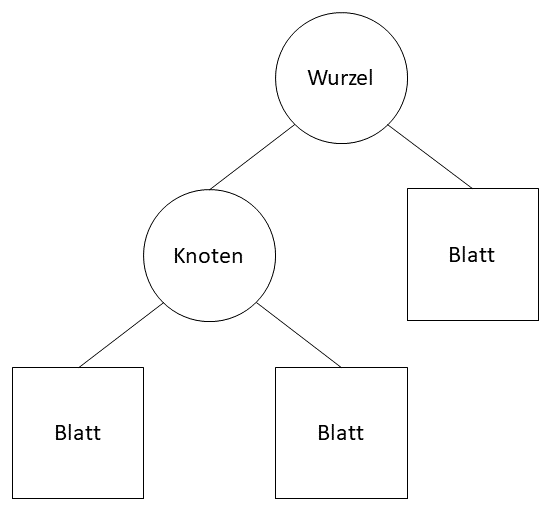
\includegraphics[width=0.5\textwidth]{images/DT}
    \caption{Grundsätzlicher Aufbau eines Decision Trees\label{fig:dt}}
\end{figure}

Eine Besonderheit von Decision Trees stellen sogenannte Random Forests dar. Diese beschreiben eine Lernmethode von Klassifikatoren, bei der mehrere einzelne Decision Trees gleichzeitig erzeugt werden und deren Ergebnisse anschließen aggregiert werden \cite{Alam2013}. Dazu erhält jeder Decision Tree eine Teilmenge der Eingabemenge des Datensets \cite{Alam2013}. Random Forests eigenen sich besonders zur Anwendung, wenn viele Attribute im Datenset vorhanden sind \cite{Alam2013}.

\subsubsection*{k-Nearest-Neighbors}
Ein k-Nearest-Neighbor-Klassifikator (deutsch: k-nächste-Nachbarn) basiert auf zwei Konzepten \cite{Zhang2016}. Das erste basiert auf der Abstandsmessung zwischen den Werten der zu klassifizierenden Datenmenge und den Werten der Attribute des Datensets \cite{Zhang2016}. Die Abstandmessung erfolgt in der Regel durch die Berechnung der Euklidischen Distanz (siehe Abbildung XX). Das zweite Konzept bildet der Parameter k, der angibt, wie viele nächste Nachbarn zum Vergleich der zuvor berechneten Abstände in Betracht gezogen werden. Bei einem k > 1 wird diejenige Zielklasse gewählt, deren Auftreten innerhalb der nächsten Nachbarn überwiegt.

\begin{figure}[]
    \centering
    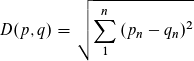
\includegraphics[width=0.4\textwidth]{images/EUKLID}
    \caption{Formel zur Berechnung der Euklidischen Distanz (n = Anzahl der Attribute)\label{fig:euklid}}
\end{figure}

\subsubsection*{Künstliche neuronale Netze}
Künstliche neuronale Netze (KNN) verwenden nicht-lineare Funktionen zur schrittweisen Erzeugung von Beziehungen zwischen der Eingabemenge und den Zielklassen durch einen Lernprozess \cite{Linder2004}. Sie sind angelehnt an die Funktionsweise von biologischen Nervensystemen und bestehen aus einer Vielzahl von einander verbundenen Berechnungsknoten, den Neuronen \cite{OShea2015}. Der grundsätzliche Aufbau eines künstlichen neuronalen Netzes kann in Abbildung XX eingesehen werden. Der Lernprozess besteht aus zwei Phasen - einer Trainingphase und einer Recall-Phase \cite{Linder2004}. In der Trainingsphase werden die Eingabedaten, meist als multidimensionaler Vektor, in den Input-Layer geladen und anschließend an die Hidden-Layer verteilt \cite{OShea2015}. In den Hidden-Layers werden dann Entscheidungen anhand der Beziehungen zwischen den Eingabedaten und Zielklassen sowie die den Verbindungen zuvor zugewiesenen Gewichtsfaktoren getroffen \cite{Linder2004}. 
\textbf{HIER!}
\cite{Linder2004}

\begin{figure}[]
    \centering
    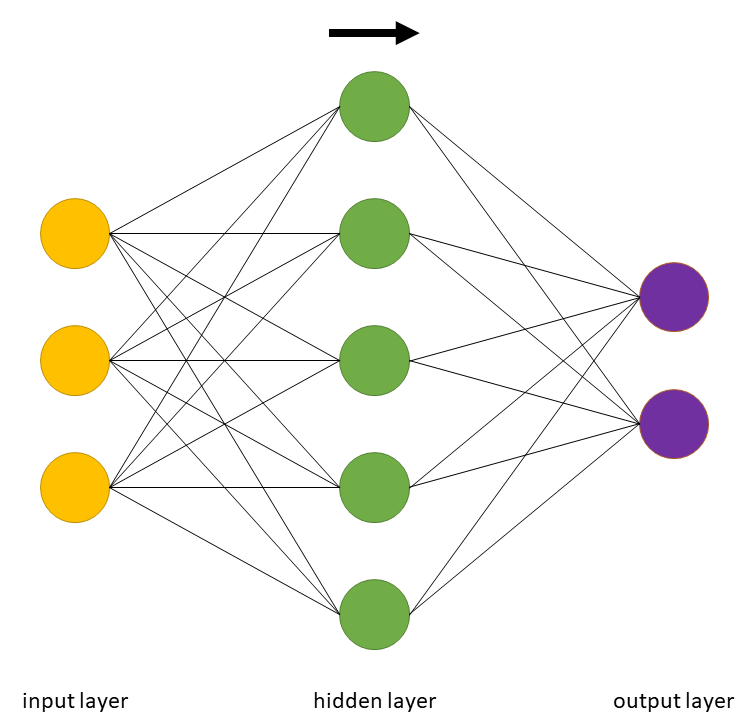
\includegraphics[width=0.6\textwidth]{images/ANN}
    \caption{Grundsätzlicher Aufbau eines KNN mit 4 Input-Neuronen, 5 Hidden-Neuronen und 2 Output-Neuronen\label{fig:ann}}
\end{figure}

\textbf{HIER!}

\subsubsection*{Na\"{\i}ve Bayes}
Na\"{\i}ve-Bayes-Klassifikatoren zählen zu den linearen Klassifikatoren und basieren auf dem Satz von Bayes. Die Bezeichnung "naiv" erhält der Klassifikator durch die Annahme, dass Attribute der Eingabemenge unabhängig voneinander sind (diese Annahme wird häufig verletzt, dennoch erzielt der Klassifikator eine hohe Performanz) \cite{Raschka2014}. Der Klassifikator gilt als effizient, robust, schnell und einfach implementierbar \cite{Raschka2014}. Die zur Durchführung einer Klassifikation mittels Na\"{\i}ve Bayes benötigte Formel nach Thomas Bayes ist in Abbildung XX samt Erläuterung aufgeführt.

\begin{figure}[]
    \centering
    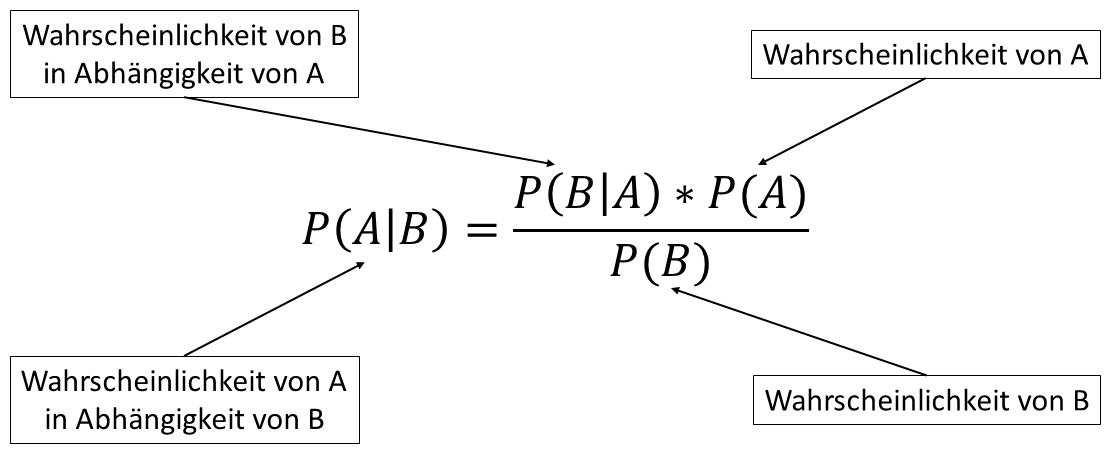
\includegraphics[width=0.7\textwidth]{images/NB}
    \caption{Satz von Bayes als Grundlage des Na\"{\i}ve-Bayes-Klassifikators\label{fig:nb}}
\end{figure}

Es existiert zudem eine Mehrzahl an Varianten des Na\"{\i}ve-Bayes-Klassifikators, die verschiedene Annahmen über die Verteilung der Attribute der Eingabemenge machen. Beispiele dafür sind der Gauß'sche-Na\"{\i}ve-Bayes (normalverteilte Attribute), der multinomiale Na\"{\i}ve-Bayes (multinomiale Verteilung der Attribute) sowie der Bernoulli-Na\"{\i}ve-Bayes (unabhängige binäre Attribute).

\subsubsection*{Logistic Regression}
Logistische Regressions-Klassifikatoren basieren auf dem mathematischen Konzept des Logits, welcher den natürlichen Logarithmus eines Chancenverhältnisses beschreibt \cite{Peng2002}. Am besten geeignet ist dieser Klassifikator für eine Kombination aus kategorischen oder kontinuierlichen Eingabedaten und kategorischen Zielklassen \cite{Peng2002}.

\textbf{HIER}

\subsubsection*{Stochastic Gradient Descent}
\cite{Bottou2010}

\subsubsection*{Support Vector Machines}
Support Vector Machines verfolgen das Ziel, linear separierbare Klassen 
\cite{Tzotsos2006}

\section{Analyse des Testprozesses}

\textbf{KONFIGURATION DER KLASSIFIKATOREN ERLÄUTERN + FINALE KONFIG ALS TABELLE}\\\textbf{SMOTE}

Im weiteren Verlauf dieses Abschnitts und im Rahmen der Evaluation im folgenden Kapitel, werden die Namen der Klassifikatoren auf Abbildungen abgekürzt. Die Abkürzungen können Tabelle XX entnommen werden.

\begin{table}
\centering
\caption{Zuordnung der verwendeten Abkürzungen}
\label{tab:abbs}
\resizebox{\linewidth}{!}{%
\begin{tabular}{|>{\centering\hspace{0pt}}p{0.15\linewidth}>{\hspace{0pt}}p{0.329\linewidth}|>{\centering\hspace{0pt}}p{0.15\linewidth}>{\hspace{0pt}}p{0.362\linewidth}|} 
\hline
\textbf{Abkürzung}  & \textbf{Klassifikator}  & \textbf{Abkürzung}  & \textbf{Klassifikator}  \\ 
\hline
DT / J48 & Decision Trees & RC & Ridge Classifier \\
KNN & k-Nearest-Neighbor & RF & Random Forest \\
LR & Logistic Regression & SGD & Stochastic Grandient Descent \\
NB & Na\"{\i}ve Bayes & SVM & Support Vector Machines \\
NN & künstliche neuronale Netze &  &  \\
\hline
\end{tabular}
}
\end{table}

Die Analyse des Testprozesses zeigte zudem, dass das dateibasierte Datenset stark unbalanciert hinsichtlich der Zielklasse ist. Mit einem Wert von etwa 98\% existieren weitaus mehr Einträge, die dem Label \glqq fehlerfrei\grqq{} zugeordnet sind. Balanciertheit, also ein ausgeglichenes Verhältnis (50:50 ist im binären Fall nicht zwingend notwendig) innerhalb der Zielklassen, ist jedoch eine Voraussetzung für das korrekte Erlernen der meisten Klassifikatoren. Eine Nichtbeachtung dieses Problem kann zu einer irreführenden Accuracy führen, da die meisten Datensätze korrekt der überrepräsentierten Klasse zugeordnet werden. Als Lösung dieses Problems wurde der sogenannte SMOTE-Algorithmus auf das dateibasierte Datenset angewendet \cite{Chawla2002}. Der Algorithmus, dessen Akronym für \textbf{S}ynthetic \textbf{M}inority \textbf{O}ver-sampling \textbf{Te}chnique steht, führt ein Oversampling der unterrepräsentierten Klasse durch \cite{Chawla2002}. Anhand von nächste-Nachbarn-Berechnungen auf Basis der Euklidischen Distanz zwischen den Attributwerten der einzelnen Datensätze des Datensets, werden neue synthetische Datensätze hinzugefügt (Oversampling), sodass sich die Anzahl der Datensätze der relevanten Klasse erhöht \cite{Chawla2002}. Im hier durchgeführten Fall wurde der Prozentsatz für die Generierung der synthetischen Datensätze auf 3000 festgelegt, sodass für jeden vorhandenen Datensatz der unterrepräsentierten Klasse 30 zusätzliche synthetische Datensätze erzeugt wurden. So konnte der Anteil der Datensätze mit dem Label \glqq fehlerhaft\grqq{} auf etwa 27\% erhöht werden. In Abbildung XX ist dargestellt, welchen Einfluss die Anwendung des SMOTE-Algorithmus auf die Accuracies der Klassifikatoren des datenbasierten Datensets im Rahmen des Testprozesses hatte. Das mit \glqq vorher\grqq{} deklarierte Diagramm zeigt, dass nahezu alle Klassifikatoren eine Accuracy von nahezu 100\% besitzen, was das zuvor beschriebene Problem widerspiegelt. Das Diagramm, welches die Testergebnisse nach Anwendung des SMOTE-Algorithmus darstellt, weist hingegen wesentlich realistischere Accuracies auf.


\begin{figure}[]
    \centering
    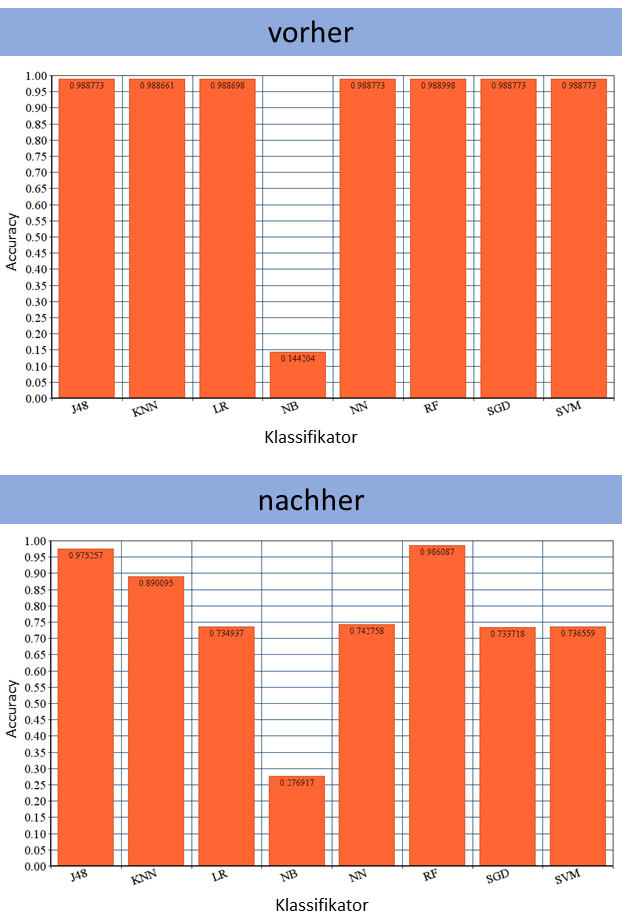
\includegraphics[width=0.8\textwidth]{images/smoted}
    \caption{Vergleich der Accuracies je Klassifikator vor und nach der Anwendung des SMOTE-Algorithmus\label{fig:smoted}}
\end{figure}

\begin{figure}[]
    \centering
    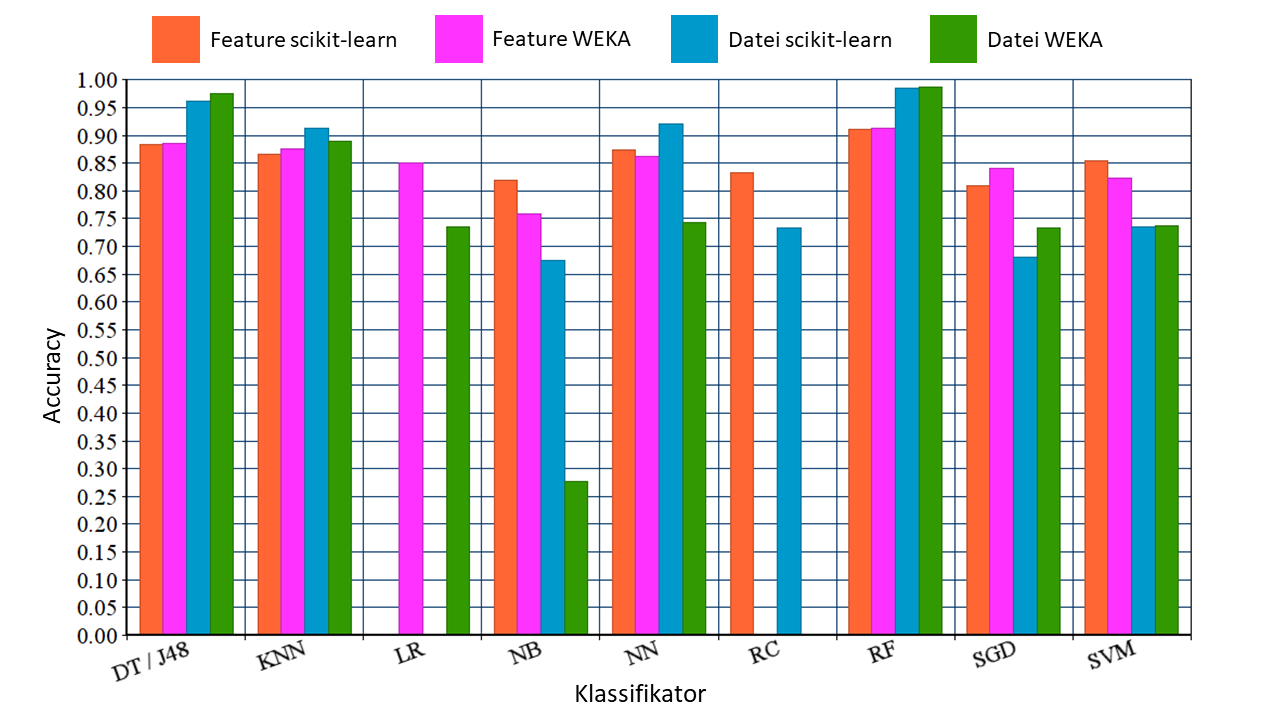
\includegraphics[width=\textwidth]{images/Vergleich1}
    \caption{Vergleich der Klassifikatoren und Werkzeuge im Hinblick auf ihre Accuracies\label{fig:vergl1}}
\end{figure}

\cleardoublepage